\section{Statistiken}
  \subsection{Erzeugung von Daten}

    Wir haben in unserem Fall diese Scripte f"ur die am Ende des Kapitels 
    angeh"angten Statistiken verwendet.\\
    \begin{code}[caption={Script zur Datenerzeugung},label=listing_datacreation]
#!/usr/bin/env ruby
require 'open3'

File.delete(ARGV[1]) if File.exists?(ARGV[1])
ARGV[2].to_i.times do |i|
  options = "--algorithm #{ARGV[0]} --threads 8 --number 10 --points #{i+4}" <<
    " --database #{ARGV[1]}"
  options + " --boundingbox #{ARGV[3]}" if ARGV[3]
  options + " --radius #{ARGV[4]}" if ARGV[4]
  options + " --runs #{ARGV[5]}" if ARGV[5]
  `java -jar polygonsSWP-bin.jar #{options}`
end
    \end{code}\\
    Bei diesem Script k"onnen wir mithilfe des ersten Parameters angeben 
    welcher Algorithmus verwendet soll, mit dem zweiten in welche Datei 
    geschrieben werden soll und mit dem dritten bis zu welcher Punktanzahl 
    Polygone generiert werden soll.\\
    Mit den weiteren Parametern kann man gr"o"se der Boundingbox, Radius 
    des initial Kreises bei Virmani's Velocity und die anzahl der Iteration
    pro Durchlauf bei Virmani's Velocity bestimmen. Sie haben allerdings
    bis auf die Boundingbox keine Relevanz f"ur die anderen Algorithmen.
  \subsection{Visualisierung der Daten}
    Zur Visualisierung der Daten haben wir ein Tool namens \enquote{plotty} in 
    \enquote{Ruby} entwickelt mit dem es m"oglich ist die SQL-Datenbank nach in
    ihr enthaltenen Daten mit SQL-Queries zu durchsuchen und die Ergebnisse 
    dieser Queries automatisiert von \enquote{GNUPlot} visualisieren zu lassen.\\
    Hierbei verwendet wir eine eigens entwickelte Konfigurationssyntax, die 
    in Form von einer YAML-Datei an \enquote{plotty} "ubergeben wird.\\
    Die Konfigurationsdateien sind wie folg strukturiert:\\
        \begin{code}[caption={Plotkonfiguration},label=listing_plotconfiguration]
sp:
  data: 
    - space.db
  adapter: sqlite
  doc_title: Space Partitioning
  diagram0:
    title: Time for Creation
    xlabel: points n
    ylabel: time in s
    style: lines
    query: |
      select number_of_points as numberOfPoints, sum(time_for_creating_polygon) as 
      timeForCreation from Statistic group by number_of_points
rpa:
  data: 
    - rpa.db
  adapter: sqlite
  doc_title: Random Polygon Algorithm
  diagram0:
    title: Time for Creation
    xlabel: points n
    ylabel: time in s
    style: lines
    query: |
      select number_of_points as numberOfPoints, sum(time_for_creating_polygon) as 
      timeForCreation from Statistic group by number_of_points
velo_good:
  data: 
    - velo_good.db
  adapter: sqlite
  doc_title: Virmani's Velocity
  diagram0:
    title: Time for Creation
    xlabel: points n
    ylabel: time in s
    style: lines
    query: |
      select number_of_points as numberOfPoints, sum(time_for_creating_polygon) as 
      timeForCreation from Statistic group by number_of_points
    \end{code}\\
    Als erstes gruppiert man die Konfigurationen nach dem Auswertungsthema,
    in diesem Fall sind es die drei verschiedenen Algorithmen
    \enquote{Space Partitioning}, \enquote{RPA} und 
    \enquote{Virmani's Velocity}.\\
    Nun Spezifiziert man pro Gruppierung eine Datenquelle, sowie den zu 
    verwendenen Adapter. Bis jetzt ist es zwar nur m"oglich SQLite als Adapter
    zu w"ahlen und auch nur eine SQLite Datenbank als Quelle, aber Support 
    f"ur mehrere Datenbanken sowie andere Adapter ist geplant.\\
    Als letztes spezifiziert man beliebig viele Diagramme pro Gruppierung,
    die alle aus der gleichen Datenquelle erstellt werden, sich aber durch die
    Angabe des zu verwenden SQL-Queries stark in Ausrichtung unterscheiden
    k"onnen. So ist es z.B. m"oglich nicht nur Punkte "uber Zeit abzutragen,
    sondern dies gleichzeitg f"ur Fl"cheninhalt und Umfang zu tuen. Alles
    mit einem Aufruf von \enquote{plotty}.\\
    Auserdem kann man durch ein Latex Template automatisiert die Art und Weise 
    steuern wie die fertigen Diagramme eingebunden werden sollen. Hierzu benutzt
    man \enquote{!!title!!} als sp"ateren Dokumententitel und 
    \enquote{!!diagrams!!} f"ur die erstellten Diagramme.\\
    Der Aufruf von \enquote{plotty} erfolgt mit den hier aufgef"uhrten
    Parametern, sowie mit einer validen Konfiguration und einem validen 
    Template.\\
    \begin{code}[caption={Plottyparameter},label=listing_plottyparameter]
Usage: plotty
    -h, --help
    -c, --conf [config] 
    -t, --template [template]
    -o, --output [out]
    \end{code}\\
    Das gesamte Projekt kann man unter \url{http://github.com/bigzed/plotty }
    herunterladen, da es zu einer eigenen Umgebung ausgearbeitet werden soll und
    nicht Teil dieses Projektes ist.
  \subsection{Diagramme}
    Die nachfolgenden Diagramme wurden mit \enquote{plotty} aus den Daten
    erstellt, die mit dem Skript in Listing~\ref{listing_datacreation} erzeugt 
    wurden.\\
    \subsubsection{Space Partioning und RPA}
      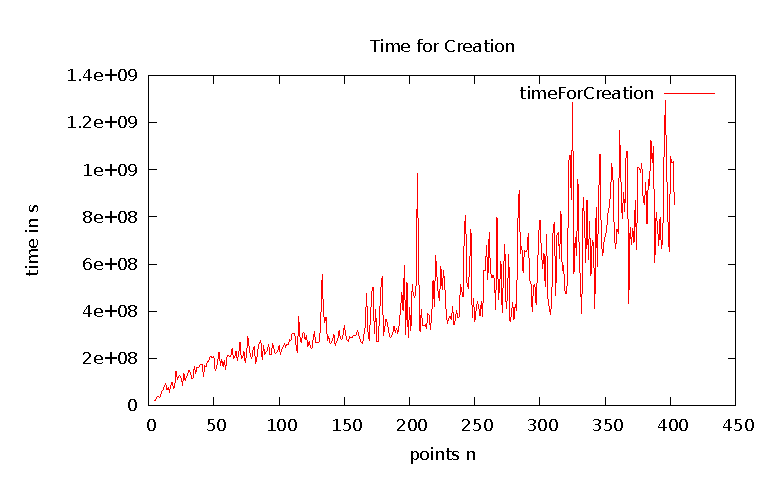
\includegraphics{img/sp_diagram_0.eps}\\
      Dieses Diagramm zeigt die ben"otigte Zeit von \enquote{Space Partioning} um 
      Polygone im Bereich von 4-400 Punkten zu erstellen. Hierbei wurden pro 
      Punktanzahl 20 Polygone erstellt um m"ogliche ausreizer negieren zu k"onnen.\\
      \includegraphics{img/rpa_diagram_0.eps}\\
      Dieses Diagram zeigt die ben"otigte Zeit von \enquote{RPA} um Polygone
      im Bereich von 4-400 Punkten zu erstellen.\\
      Man kann erkennen, das obwohl beide Algorithmen auf dem selben 8 Kern
      System mit 8GB RAM ausgewertet wurden liegt die Dauer zur Erzeugung von 
      Polygonen mit dem \enquote{RPA} bei gleichen Bedingungen zwei gr"o"sen 
      Ordnungen "uber \enquote{Space Partioning}.\\
      Allerdings sollte man f"ur eine genauere Auswertung mehr Polygone pro
      Punktanzahl erzeugen, da das Diagramm von \enquote{Space Partioning} doch
      starke Schwankungen zeigt.
    \subsubsection{Virmani's Velocity}
      Diese beiden Diagramme sind beide mit Virmani's Velocity erstellt worden,
      allerdings mit v"ollig unterschiedlichen Parametern.\\
      Der erste Plot zeigt den Algorithmus mit einer gro"sen Boundingbox 
      und verh"altnism"a"sig kleinem Initialradius f"ur die Punkte, sowie 
      nur 100 Iteration pro Durchlauf.\\
      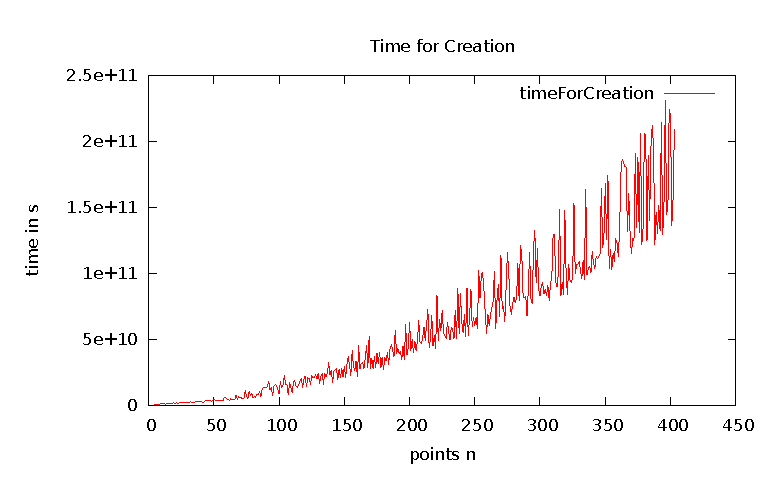
\includegraphics{img/velo_good_diagram_0.eps}\\
      Der Zweite Plot zeigt den Algorithmus mit einer ebenfalls gro"sen 
      Boundingbox und einem maximal gew"ahlten Initialradius, sowie 300 Iterationen
      pro Durchlauf.\\
      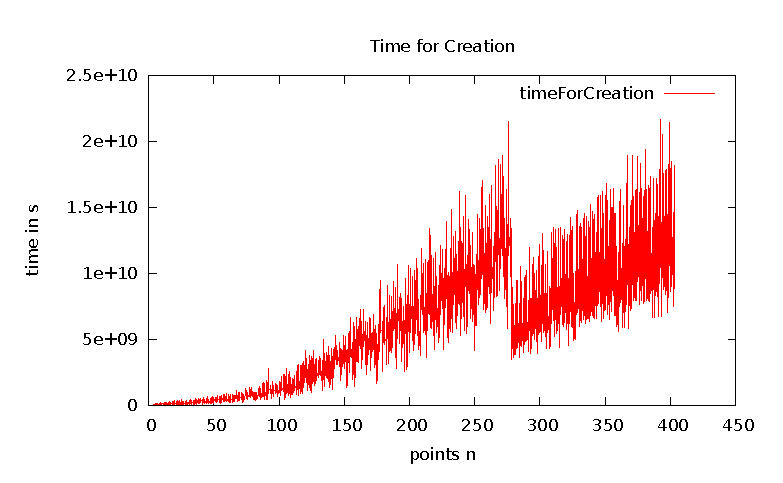
\includegraphics{img/velo_bad_diagram_0.eps}
